\documentclass[a4paper, landscape, 6pt]{article}

% --------------------------------------------------------------------------------------------------------------------------------------------------------------------------
\input{./package_and_config.tex}

\def\subject{Mathematik}
\def\semester{2. Semester}
\def\author{Michael Graber, Joshua Kohler, Sven Gahlinger, Oliver Schütz}
\def\cols{3}

% Useful packages
\usepackage{amsmath}
\usepackage{graphicx}
\usepackage[colorlinks=true, allcolors=blue]{hyperref}
\usepackage{makecell}
\usepackage{adjustbox}
\usepackage{pgfplots}

\title{Mathe 2 Cheatsheet}

\cheatsheet{
    \section{Allgemein}
    \subsubsection{Linearität}
\begin{flalign}
    &f(x) \cdot a = f(x \cdot a) \qquad \forall a \in \mathbf{R}, \forall x \in \mathbf{R}^{n}&\\
    &f(x) + f(y) = f(x + y) \qquad V_{x,y} \in \mathbf{R}^{n}&\\
    &\textbf{Lineares Beispiel: } f(x) = 3x \text{ mit } a=3,\ x=2,\ y=5&\notag\\
    &1.\ \text{Homogenitätstest: } f(2 \cdot 3) \stackrel{?}{=} 3 \cdot f(2) &\notag\\
    &\ \ \quad f(6) = 6 \cdot 3 = 18 \quad \text{vs.} \quad 3 \cdot 3 \cdot 2 = 3 \cdot 6 = 18 \quad \Rightarrow 18 = 18\ (\checkmark)&\notag\\
    &2.\ \text{Additivitätstest: } f(2) + f(5) \stackrel{?}{=} f(2+5) &\notag\\
    &\ \ \quad (3 \cdot 2) + (3 \cdot 5) = 6 + 15 = 21 \quad \text{vs.} \quad 3 \cdot 7 = 21 \quad \Rightarrow 21 = 21\ (\checkmark)&\notag\\
    &\textbf{Gegenbeispiel: } f(x) = x^2 \text{ mit } a=2,\ x=3,\ y=4&\notag\\
    &1.\ \text{Homogenitätstest: } f(3 \cdot 2) \stackrel{?}{=} 2 \cdot f(3) &\notag\\ 
    &\ \ \quad f(6) = 6^2 = 36 \quad vs. \quad 2 \cdot 3^2 = 18 \quad \Rightarrow 36 \ne 18\ (\times)&\notag\\
    &2.\ \text{Additivitätstest: } f(3) + f(4) \stackrel{?}{=} f(3+4) &\notag\\
    &\ \ \quad 3^2 + 4^2 = 9 + 16 = 25 \quad vs. \quad 7^2 = 49 \quad \Rightarrow 25 \ne 49\ (\times)&\notag
\end{flalign}


    \subsubsection{Injektiv}
$\mathbb{R} \mapsto \mathbb{R}^n \Leftrightarrow f(x) = f(y) \Rightarrow x = y$:\\
\bullet \, Jedes Element der Zielmenge höchstens einmal als Funktionswert\\
\bullet \, Alle x von $\mathbb{D}$ können genau ein y von $\mathbb{W}$ durch $f(x)$ erhalten.
$\mathbb{W}$ muss nicht aber kann aber vollständig agbedeckt sein.

\begin{minipage}{0.4\linewidth}
    % Injective Function
    \begin{tikzpicture}[
        scale=0.7,
        set/.style={ellipse, draw, minimum width=2cm, minimum height=3cm},
        element/.style={circle, fill=black, inner sep=1pt}]
    
    % Domain (left set)
    \node[set] (A) at (1.5,0) {$\mathbb{D}$};
    \node[element,label=left:$a$] (a) at (1.5,1) {};
    \node[element,label=left:$b$] (b) at (1.5,0.5) {};
    \node[element,label=left:$c$] (c) at (1.5,-0.5) {};
    
    % Codomain (right set)
    \node[set] (B) at (4,0) {$\mathbb{W}$};
    \node[element,label=right:$1$] (1) at (4,1) {};
    \node[element,label=right:$2$] (2) at (4,0.5) {};
    \node[element,label=right:$3$] (3) at (4,-0.5) {};
    \node[element,label=right:$4$] (4) at (4,-1) {};
    
    % Arrow mappings
    \draw[->,blue] (a) to[bend left] (1);
    \draw[->,red] (b) to (2);
    \draw[->,green!70!black] (c) to[bend right] (3);
    \end{tikzpicture}
\end{minipage}
\hfill
\begin{minipage}{0.49\linewidth}
    % Injective function (e^x)
    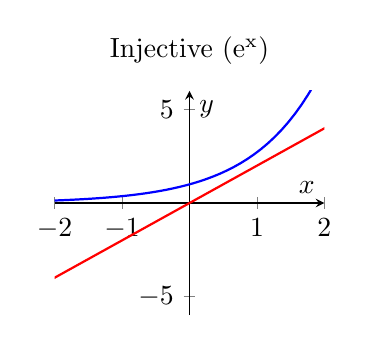
\begin{tikzpicture}
    \begin{axis}[
        scale=0.5,
        axis lines=middle,
        xlabel=\(x\),
        ylabel=\(y\),
        xmin=-2, xmax=2,
        ymin=-6, ymax=6,
        samples=100,
        title={Injective (e\textsuperscript{x})}
    ]
    \addplot[blue, thick] {exp(x)};
    \addplot[red, thick] {2*x};
    \end{axis}
    \end{tikzpicture}
\end{minipage}


\subsubsection{Surjektiv}
$\mathbb{R}^n \mapsto \mathbb{R}$:\\
\bullet \, Jedes Element der Zielmenge mindestens einmal als Funktionswert.\\
\bullet \, $\mathbb{W}$ kann durch $f(x)$ mit x von $\mathbb{D}$ vollständig abgedeckt werden.
\begin{minipage}{0.4\linewidth}
    % Surjective Function
    \begin{tikzpicture}[
        scale=0.7,
        set/.style={ellipse, draw, minimum width=2cm, minimum height=3cm},
        element/.style={circle, fill=black, inner sep=1pt}]
    
    % Domain (left set)
    \node[set] (A) at (1.5,0) {$\mathbb{D}$};
    \node[element,label=left:$a$] (a1) at (1.5,1) {};
    \node[element,label=left:$b$] (b1) at (1.5,0.5) {};
    \node[element,label=left:$c$] (c1) at (1.5,-0.5) {};
    \node[element,label=left:$d$] (d1) at (1.5,-1) {};
    
    % Codomain (right set)
    \node[set] (B) at (4,0) {$\mathbb{W}$};
    \node[element,label=right:$1$] (1) at (4,1) {};
    \node[element,label=right:$2$] (2) at (4,0.5) {};
    \node[element,label=right:$3$] (3) at (4,-0.5) {};
    
    % Arrow mappings
    \draw[->,blue] (a1) to (1);
    \draw[->,red] (b1) to (2);
    \draw[->,green!70!black] (c1) to (3);
    \draw[->] (d1) to[bend right] (3);
    \end{tikzpicture}
\end{minipage}
\hfill
\begin{minipage}{0.4\linewidth}
    % Surjective function (x^3)
    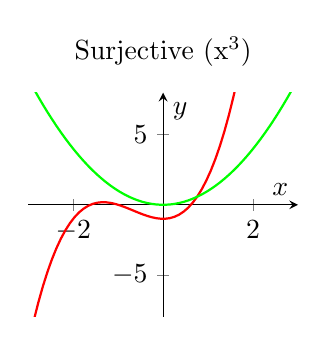
\begin{tikzpicture}
    \begin{axis}[
        scale=0.5,
        axis lines=middle,
        xlabel=\(x\),
        ylabel=\(y\),
        xmin=-3, xmax=3,
        ymin=-8, ymax=8,
        samples=100,
        title={Surjective (x\textsuperscript{3})}
    ]
    \addplot[red, thick] {x^3 + 2*x^2 - 1};
    \addplot[green, thick] {x^2};
    \end{axis}
    \end{tikzpicture}
\end{minipage}



\subsubsection{Bijektiv}
$\mathbb{R} \mapsto \mathbb{R}$\\
\bullet \, Jedes Element der Zielmenge genau einmal als Funktionswert.\\
\bullet \, Bijektive Funktionen haben eine Inverse Funktion.


\begin{minipage}{0.4\linewidth}
    % Bijective Function
    \begin{tikzpicture}[
        scale=0.7,
        set/.style={ellipse, draw, minimum width=2cm, minimum height=3cm},
        element/.style={circle, fill=black, inner sep=1pt}]
    
    % Domain (left set)
    \node[set] (A) at (1.5,0) {$\mathbb{D}$};
    \node[element,label=left:$a$] (a2) at (1.5,1) {};
    \node[element,label=left:$b$] (b2) at (1.5,0.5) {};
    \node[element,label=left:$c$] (c2) at (1.5,-0.5) {};
    
    % Codomain (right set)
    \node[set] (B) at (4,0) {$\mathbb{W}$};
    \node[element,label=right:$1$] (1) at (4,1) {};
    \node[element,label=right:$2$] (2) at (4,0.5) {};
    \node[element,label=right:$3$] (3) at (4,-0.5) {};
    
    % Arrow mappings
    \draw[->,blue] (a2) to[bend left=10] (1);
    \draw[->,red] (b2) to[bend left=0] (2);
    \draw[->,green!70!black] (c2) to[bend right=10] (3);
    \end{tikzpicture}
\end{minipage}
\hfill
\begin{minipage}{0.4\linewidth}
    % Bijective function (linear)
    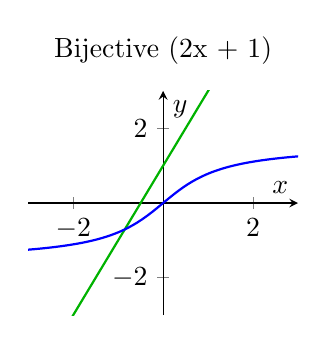
\begin{tikzpicture}
    \begin{axis}[
        scale=0.5,
        axis lines=middle,
        xlabel=\(x\),
        ylabel=\(y\),
        xmin=-3, xmax=3,
        ymin=-3, ymax=3,
        samples=100,
        title={Bijective (2x + 1)}
    ]
    \addplot[green!70!black, thick] {2*x + 1};
    \addplot[blue, thick] {rad(atan(x))};
    \end{axis}
    \end{tikzpicture}
\end{minipage}
    \section{Analysis}
    \input{../../Snippeds/Allgemein/Polynome.tex}
    \subsubsection{Hornerschema}
\textcolor{red}{Hier noch ein gutes beispiel einfügen}
Polynomial example: \( p(x) = 2x^3 + 3x^2 + 4x + 5 \) evaluated at \( x = 1 \)
\begin{minipage}{0.4\linewidth}
    \begin{tabular}{r|rrrr}
        & 2 & 3 & 4 & 5 \\ \hline
    1 & $\cdot$ & 2 $\searrow$ & 5 $\searrow$ & 9 $\searrow$ \\
        & 2 & 5 & 9 & \boxed{14} \\
    \end{tabular}
\end{minipage}
\hfill
\begin{minipage}{0.4\linewidth}
    Where factors are calculated as:
    \begin{align*}
        2 \times 1 + 3 &= 5 \\
        5 \times 1 + 4 &= 9 \\
        9 \times 1 + 5 &= 14 \\
    \end{align*} 
\end{minipage}
    \subsubsection{Nullstellen}
\begin{flalign}
    &\textbf{Mitternachtsformel}&\notag\\
    &f(x) = ax^2 + bx +c \Rightarrow x_1/x_2 = \frac{-b \pm \sqrt{b^2 - 4ac}}{2a}&\label{eq:Mitternachtsformel}\\
    &\textbf{Satz über rationale Nullstelen} \text{  -  Empfohlen bei kleinen Koeffizienten } (a_n)&\notag\\
    &f(x) = \color{red} a_n \color{black} x^2 + a_{n - 1} x^{n - 1} + \cdots + a_1 x + \color{blue} a_0 \color{black} \,|\, \color{blue} a_0 \color{black} , a_1, \ldots, \color{red} a_n \color{black} \in \mathbb{Z} \quad \bf \color{orange}(a_n \ne 0)&\\
    &x_0 = \frac{P}{q} (p,q \in \mathbb{Z}, ggT(P,q) = 1) \Rightarrow \color{red} a_0 \color{black} \text{ durch P teilbar, } \color{blue} a_n \color{black} \text{ durch q teilbar}&\\
    &\Rightarrow T = \pm \frac{\text{\textcolor{blue}{Teiler von $a_0$}}}{\text{\textcolor{red}{Teiler von $a_n$}}}&\notag
\end{flalign}

    \subsection{Trigonometrie}
    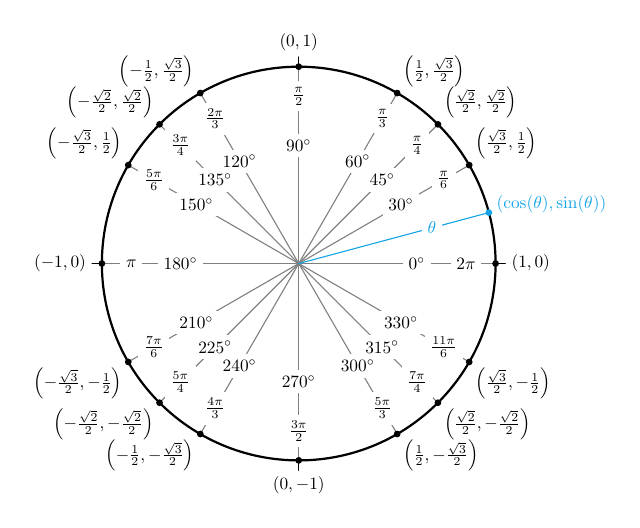
\begin{tikzpicture}[scale=2.5, transform shape, cap=round,>=latex, every node/.style={scale=0.25}] 
    % draw the coordinates
    \draw[-] (-1.05cm,0cm) -- (1.05cm,0cm);
    \draw[-] (0cm,-1.05cm) -- (0cm,1.05cm);

    % draw the unit circle
    \draw[thick] (0cm,0cm) circle(1cm);

    \foreach \x in {0,30,45,60,90,120,135,150,180,210,225,240,270,300,315,330} {
            % lines from center to point
            \draw[gray] (0cm,0cm) -- (\x:1cm);
            % dots at each point
            \filldraw[black] (\x:1cm) circle(0.4pt);
            % draw each angle in degrees
            \draw (\x:0.6cm) node[fill=white] {$\x^\circ$};
    }

    \draw[Cerulean](0cm,0cm) -- (15:1cm);
    \filldraw[Cerulean] (15:1cm) circle(0.4pt);
    \draw (15:0.7cm) node[Cerulean,fill=white] {$\theta$};
    \draw (13:1cm) node[above right,Cerulean] {$\left(\cos(\theta), \sin(\theta)\right)$};

    % draw each angle in radians
    \foreach \x/\xtext in {
        30/\frac{\pi}{6},
        45/\frac{\pi}{4},
        60/\frac{\pi}{3},
        90/\frac{\pi}{2},
        120/\frac{2\pi}{3},
        135/\frac{3\pi}{4},
        150/\frac{5\pi}{6},
        180/\pi,
        210/\frac{7\pi}{6},
        225/\frac{5\pi}{4},
        240/\frac{4\pi}{3},
        270/\frac{3\pi}{2},
        300/\frac{5\pi}{3},
        315/\frac{7\pi}{4},
        330/\frac{11\pi}{6},
        360/2\pi}
            \draw (\x:0.85cm) node[fill=white] {$\xtext$};

    \node[right] at (0:1.05cm) {$\left(1,0\right)$};
    \node[above] at (90:1.05cm) {$\left(0,1\right)$};
    \node[left] at (180:1.05cm) {$\left(-1,0\right)$};
    \node[below] at (270:1.05cm) {$\left(0,-1\right)$};

    \foreach \x/\xtext/\y in {
        150/-\frac{\sqrt{3}}{2}/\frac{1}{2},
        135/-\frac{\sqrt{2}}{2}/\frac{\sqrt{2}}{2},
        120/-\frac{1}{2}/\frac{\sqrt{3}}{2}}
            \draw (\x:1cm) node[above left] {$\left(\xtext,\y\right)$};

    
    \foreach \x/\xtext/\y in {
        30/\frac{\sqrt{3}}{2}/\frac{1}{2},
        45/\frac{\sqrt{2}}{2}/\frac{\sqrt{2}}{2},
        60/\frac{1}{2}/\frac{\sqrt{3}}{2}}
            \draw (\x:1cm) node[above right] {$\left(\xtext,\y\right)$}; 
    
    \foreach \x/\xtext/\y in { 
        210/-\frac{\sqrt{3}}{2}/-\frac{1}{2},
        225/-\frac{\sqrt{2}}{2}/-\frac{\sqrt{2}}{2},
        240/-\frac{1}{2}/-\frac{\sqrt{3}}{2} }
            \draw (\x:1cm) node[below left] {$\left(\xtext,\y\right)$};

    \foreach \x/\xtext/\y in {
        330/\frac{\sqrt{3}}{2}/-\frac{1}{2},
        315/\frac{\sqrt{2}}{2}/-\frac{\sqrt{2}}{2},
        300/\frac{1}{2}/-\frac{\sqrt{3}}{2}}
            \draw (\x:1cm) node[below right] {$\left(\xtext,\y\right)$};
\end{tikzpicture}
    \input{../../Snippeds/Tigonometrie/unitcircle_2.tex}
    \begin{tabularx}{\linewidth}{|X|X|X|X|}
    \hline
    \textbf{Sin} & \textbf{Cos} & \textbf{Tan} & \textbf{Cot}\\
    \hline
    \textbf{G} & \textbf{A} & \textbf{G} & \textbf{A}\\
    \hline
    \textbf{H} & \textbf{H} & \textbf{A} & \textbf{G}\\
    \hline
\end{tabularx}

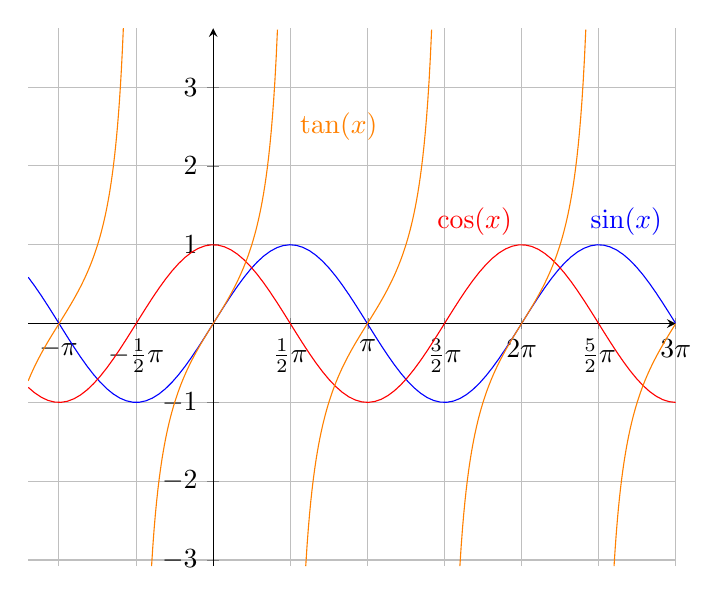
\begin{tikzpicture}
\begin{axis}[enlargelimits=false,
             axis lines=middle,
             scale=1.2,
             xtick={-3.15159, -1.57080, 0,
                     1.57080,  3.15159, 4.71239,
                     6.28318,  7.85398, 9.42478 }, 
             xticklabels={$-\pi$, $-\frac{1}{2}\pi$, 0,
                          $\frac{1}{2}\pi$, $\pi$, $\frac{3}{2}\pi$,
                          $2\pi$, $\frac{5}{2}\pi$, $3\pi$ },
             ytick={-3,-2,-1,0,1,2,3},
             grid=major, % only a grid on the defined ticks
             samples=100 % number of points
             ]
 
  % sin
  \addplot[blue,no marks,domain=-1.2*pi:3*pi]{sin(deg(x))}; % deg to convert radians
  \node[right=10pt,above] at (axis cs:5*pi/2,1){\color{blue}$\sin(x)$};
 
  % cos
  \addplot[red,no marks,domain=-1.2*pi:3*pi] {cos(deg(x))};
  \node[above left] at (axis cs:2*pi,1){\color{red}$\cos(x)$};
 
  % tan, multiple parts because of singularities
  \addplot[orange,no marks,domain=-1.2*pi:-0.583*pi, ]{tan(deg(x))};
  \addplot[orange,no marks,domain=-0.4*pi:5*pi/12,   ]{tan(deg(x))};
  \addplot[orange,no marks,domain=27*pi/45:17*pi/12, ]{tan(deg(x))};
  \addplot[orange,no marks,domain=1.6*pi:29*pi/12,   ]{tan(deg(x))};
  \addplot[orange,no marks,domain=2.6*pi:36*pi/12,   ]{tan(deg(x))};
  \node[right] at (axis cs:pi/2,2.5){\color{orange}$\tan(x)$};
 
\end{axis}
\end{tikzpicture}
    \subsection{Integrale}
    \subsubsection{Integrationsgrenzen tauschen}
Satz von Fubini
    \subsubsection{Substitution}
\textbf{Normale Substitution}\\
\begin{flalign}
    \int_{a}^{b} f(g(x)) dx \quad | \quad u(x) = g(x) \quad &| \quad u'(x) = g'(x) \quad | \quad du = u'(x)\cdot dx \notag&\\
    \int_{u(a)}^{u(b)} u(x) \frac{1}{u'(x)} \,du \quad &| \quad dx = \frac{1}{u'(x)} \,du&\label{eq:Substitution}\\\notag
\end{flalign}
Wenn nach einer Substitution noch ein x in der Gleichung vorhanden ist, muss dieses in ein u umgewandelt werden.

\begin{flalign}
    \int \frac{e^{2x}}{1+e^{2}} \,dx \quad | \quad u = 1 + e^{x} \quad &| \quad u' = e^{x} \quad | \quad du = e^{x} \,dx \Leftrightarrow du = \frac{1}{e^{x}}&\notag\\
    \int \frac{e^{2x}}{u} \cdot \frac{1}{e^{x}} \,du = \int \frac{e^{x}}{u} \,du \quad &| \quad u = 1 + e^{x} \Leftrightarrow e^{x} = u - 1&\notag\\
    \int \frac{u - 1}{u} \,du = \int \frac{u}{u} - \frac{1}{u} \,du &= \int 1 - \frac{1}{u} \,du = \underline{\underline{u - \ln|u| + c}} &\notag
\end{flalign}\\

\textbf{Umgekehrte Substitution (Example)}\\

\begin{flalign}
    \int_{0}^{1} \sqrt{1 - x^2}\, dx \quad &| \quad x = \sin{u} \notag \quad | \quad x' = \cos{u} \notag&\\
    \int_{0}^{\frac{\pi}{2}} \sqrt{1 - \sin^2{u}} \cdot \cos{u}\,du \quad &| \quad dx = \cos{u}\, du \Leftrightarrow   du = \frac{1}{\cos{u}}\, dx \notag&\\
    \int_{0}^{\frac{\pi}{2}} \cos^2{u}\, du \quad =& \quad \left[\frac{u}{2} +  \frac{\sin{2u}}{4}\right]_{0}^{\pi/2} = \frac{\pi}{4} + 0 = \frac{\pi}{4}&\notag
\end{flalign}
    % https://en.wikipedia.org/wiki/List_of_integrals_of_trigonometric_functions#Integral_over_a_full_circle
\subsubsection{Standardintegrale}
\begin{multicols}{2}
    \begin{flalign}
        &\textbf{Standartintegrale}&\notag\\
        &\int m \,dx = m \cdot x + q&\\
        &\int a^{x} \,dx = \frac{a^{x}}{\ln{x}} + c&\\
        &\int{e^{x}} \,dx = e^x&\\ 
        &\int{x^{p}} \,dx = \frac{1}{p+1} \cdot x^{p+1} + c \quad n \ne -1&\\
        &\int{x^{-1}} \,dx = \int{\frac{1}{x}} \,dx = \ln|x| + c&\\
        &\int_{x_0}^{x_E}{x^{-1}} \,dx = \int{\frac{1}{x}} \,dx = \ln{\frac{x_E}{x_0}}&
    \end{flalign}
    \begin{flalign}
        &\textbf{Sinus}&\notag\\
        &\int{\sin{x} \cdot \cos{x}}\, dx = \frac{1}{2} \cdot \sin^2{x} + c&\\
        &\int{\sin^2{x}} \,dx = \frac{1}{2} (x - \sin{x} \cdot \cos{x}) + c&\\
        &\int{\sinh{x}} \,dx = \cosh{x} + c&\\
        &\textbf{Cosinus}&\notag\\
        &\int{\frac{1}{\cos^2{x}} \,dx} = \int{1 + \tan^2{x}}&\notag\\
        & = \tan{x} + c&\\
        &\int{\cosh{x}}\,dx = \sinh{x} + c&\\
        &\int{\cot{x}}\, dx = \frac{1}{\tan{x}} + c&\notag\\
        &= \ln|\sin{x}| + c = \frac{\cos{x}}{\sin{x}} + c&\\
        &\int{\coth{x}}\, dx = \frac{\cosh{x}}{\sinh{x}} + c&\\
        &\textbf{Tangents}&\notag\\
        &\int{\tan{x}}\, dx = \frac{1}{\cot{x}} + c&\notag\\
        & = -\ln|\cos{x}| + c = \frac{\sin{x}}{\cos{x}} + c&\\
        &\int{\tanh{x}}\, dx = \frac{\sinh{x}}{\cosh{x}} + c&\\
        &\int{\frac{1}{1 + x^2}} \,dx = \arctan{x}&
    \end{flalign}
\end{multicols}


    \subsubsection{Integralfläche berechnen (analytisch)}
Sobald sich Funktionen schneiden, muss das Integral aufgeteilt werden.
Wenn die Fläche über/unter der X-Achse berechnet werden soll, kann diese als Funktion $g(x) = 0$ angesehen werden.

\begin{flalign}
    A = \int_{a}^{b}{|f(x) - g(x)|} \,dx \label{eq:Calculate_area}
\end{flalign}

\textcolor{red}{Scale Plot and make a better example}
\begin{center}
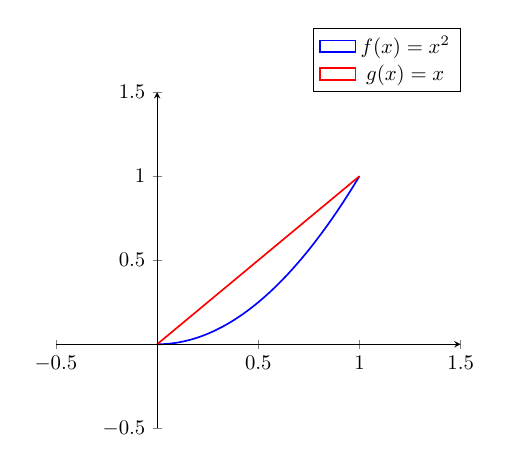
\begin{tikzpicture}[
    scale=0.75
    ]
    \begin{axis}[
        axis lines = middle,
        xmin = -0.5, xmax = 1.5,
        ymin = -0.5, ymax = 1.5,
        domain = 0:1,
        samples = 100,
        fill=blue!20,
        area style,
        legend style={at={(1,1)}, anchor=south east},
    ]
    \addplot[blue, thick] {x^2};
    \addplot[red, thick] {x};
    % \addplot[blue!20] fill between[of={x^2}, and={x}]; here is some compiling problem which I couldn't solve at the moment
    \legend{$f(x) = x^2$,$g(x) = x$}
    \end{axis}
\end{tikzpicture}
\end{center}

\textbf{Anleitung}
\begin{enumerate}
    \item Funktionen gleich setzen, um Nullstellen zu berechnen
    \item Integrale bilden
    \item Berechnen
\end{enumerate}
    \subsubsection{Partialle Integration}
\textbf{Formel}\\
\begin{flalign}
    &\int f(x) \cdot g(x) \,dx&\notag\\
    &\Rightarrow \sum_{k=0}^{n-1}{(-1)^{k} \cdot f^{k}(x) \cdot g^{-1-k}(x) + (-1)^n \int f^{n}(x) \cdot g^{-n}(x) \,dx}&\\
    &\int{f(x) \cdot g(x)} \,dx = F(x) \cdot g(x) - \int{F(x) \cdot g(x)} \,dx &
\end{flalign}
\begin{tabular}{r|cc}
    Vorzeichen & Differenzieren & Integrieren\\
    \hline
    + & $\tikzmarknode{D0}{f}$ & g\\
    - & $\tikzmarknode{D1}{f^{1}}$ & $\tikzmarknode{I1}{g^{-1}}$\\
    + & $\tikzmarknode{D2}{f^{2}}$ & $\tikzmarknode{I2}{g^{-2}}$\\
    $\pm$ & $\tikzmarknode{D3}{\vdots}$ & $\tikzmarknode{I3}{\vdots}$\\
    $(-1)^{n-1}$ & $\tikzmarknode{D4}{f^{n-1}}$ & $\tikzmarknode{I4}{g^{-n+1}}$\\
    $(-1)^{n}$ & $\tikzmarknode{D5}{f^{n}}$ & $\tikzmarknode{I5}{g^{-n}}$\\
\end{tabular}

\begin{tikzpicture}[overlay, remember picture]
    \draw[->] (D0) to (I1);
    \draw[->] (D1) to (I2);
    \draw[->] (D2) to (I3);
    \draw[->] (D3) to (I4);
    \draw[->] (D4) to (I5);
    \draw[->] (D5) to (I5);
\end{tikzpicture}

    \subsubsection{Volumenintegral berechnen}
\begin{flalign}
    &V = \pi \int_{a}^{b}{f(x)^{2}} \,dx \label{eq:Rotationsvolumen}&
\end{flalign}

\textbf{Anleitung}
\begin{enumerate}
    \item Rotation um Y-Achse \rightarrow \, Umkehrfunktion bestimmen
    \item Mit der Formel \ref{eq:Rotationsvolumen} das Volumen berechnen
\end{enumerate}
    \section{Komplexe Zahlen}
    \subsubsection{Komplexe Zahlen}
\textbf{Allgemeines Komplexe Zahlen}\\

\begin{minipage}{0.4\linewidth}
    \begin{flalign}
        &i^2 = -1&
    \end{flalign}
\end{minipage}
\hfill
\begin{minipage}{0.4\linewidth}
    \begin{flalign}
        &\textbf{Arithmetische Form}&\notag\\
        &z = x + y \cdot i&
    \end{flalign}
\end{minipage}
\begin{multicols}{2}
    \begin{itemize}
        \item Realteil von $z:\\
         \Re{z}$:= x 
        \item Imaginärteil von $z: \\
        \Im{z}$:= y\\
        \item Betrag von $z$:\\
        $|z|:= \sqrt{x^2 + y^2}$
        \item Komplex-Konjugierte von $z: z^*:= x-y \cdot i$
    \end{itemize}
    
\end{multicols}
\begin{flalign}
    &\textbf{Addition}&\notag\\
    &z_1 + z_2 = x_1 + x_2 + (y_1 + y_2) \cdot i&\\
    &\textbf{Subtraktion}&\notag\\
    &z_1 - z_2 = x_1 - x_2 + (y_1 - y_2) \cdot i&\\
    &\textbf{Multiplikation}&\notag\\
    &z_1 \cdot z_2 = x_1 \cdot x_2 - y_1 \cdot y_2 + (x_1 \cdot y_2 + x_2 \cdot y_1) \cdot i&\\
    &\textbf{Division}&\notag\\
    &\frac{z_1}{z_2} = \frac{x_1 \cdot x_2 + y_1 \cdot y_2}{x_{2}^{2} + y_{2}^{2}} + \frac{x_2 \cdot y_1 - x_1 \cdot y_2}{x_{2}^{2} + y_{2}^{2}} \cdot i&\\
    &\textbf{Betrag und Konjugation}&\notag\\
    &z \cdot z^* = |z|^2&\\
    &\textbf{Komplexe aus dem Nenner bringen}&\notag\\
    &\frac{z_1}{z_2} = \frac{z_1 \cdot z_2^*}{|z_2|^2} = \frac{(x_1 + y_1i)(x_2 - y_2i)}{x_2^2 + y_2^2}&\
\end{flalign}
\begin{multicols}{2}
    \begin{itemize}
        \item $|z_1 \cdot z_2| = |z_1| \cdot |z_2|$
        \item $|\frac{z_1}{z_2}| = \frac{|z_1|}{|z_2|}$
        \item \textbf{Dreiecks-Ungleichung}\\
        $|z_1 + z_2| \leq |z_1| + |z_2|$\\
        $|z_1 - z_2| \ge |z_1| - |z_2|$
    \end{itemize}
\end{multicols}
    

\subsubsection{Koordinaten Arten}
\begin{flalign}
    &\textbf{Kartesische Koordinaten}& \notag \\
    &z = x + iy &\\[1ex]
    &\textbf{Polarkoordinaten} & \notag \\
    &\text{Umrechnung kartesisch} \to \text{polar:} & \notag \\
    &r = \sqrt{x^2 + y^2} & \notag \\
    &\varphi = \arctan\left(\frac{y}{x}\right) \quad (x \neq 0) & \notag \\[1ex]
    &\textbf{Komplexe Polarform} & \notag \\
    &\operatorname{cis} \varphi = \cos \varphi + i \sin \varphi & \notag \\
    &z = r \operatorname{cis} \varphi = r(\cos \varphi + i \sin \varphi) & \label{eq:polarform} \\[1ex]
    &\textbf{Euler-Form} & \notag \\
    &z = re^{i\varphi} \quad \text{(äquivalent zur Polarform)} & \label{eq:euler}
\end{flalign}

\begin{flalign}
    &x = r \cdot \cos{\phi} \quad|\quad y = r \cdot \sin{\phi}&\\
    &\varphi = \arctan{\frac{x}{y}}&\\
    &z = re^{i\varphi} = x + iy = r\cdot \operatorname{cis}{\varphi}&
\end{flalign}
    \[
\arg(z) =
\begin{cases} 
    0                                                & \text{if } \Re(z) \geq 0 \land \Im(z) = 0 \quad | \quad \text{CASE 1}\\
    \arctan\left(\frac{\Im(z)}{\Re(z)}\right)        & \text{if } \Re(z) > 0 \land \Im(z) > 0 \quad | \quad \text{CASE 2}\\
    \frac{\pi}{2}                                    & \text{if } \Re(z) = 0 \land \Im(z) > 0 \quad | \quad \text{CASE 3}\\
    \arctan\left(\frac{\Im(z)}{\Re(z)}\right) + \pi  & \text{if } \Re(z) < 0 \qquad \qquad \qquad \quad| \quad \text{CASE 4}\\
    \pi                                              & \text{if } \Re(z) < 0 \land \Im(z) = 0 \quad | \quad \text{CASE 5}\\
    \frac{3\pi}{2}                                   & \text{if } \Re(z) = 0 \land \Im(z) < 0 \quad | \quad \text{CASE 6}\\
    \arctan\left(\frac{\Im(z)}{\Re(z)}\right) + 2\pi & \text{if } \Re(z) > 0 \land \Im(z) < 0 \quad | \quad \text{CASE 7}
\end{cases}
\]

\begin{center}
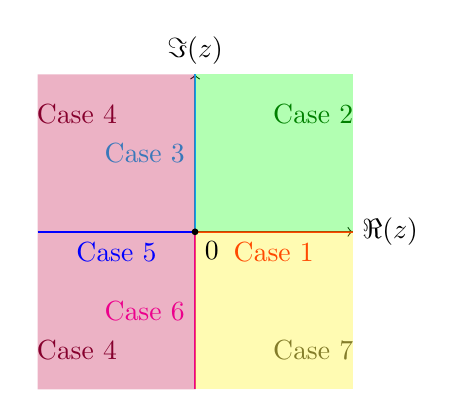
\begin{tikzpicture}[scale=1]
    % Axes
    \draw[->] (-2,0) -- (2,0) node[right] {$\Re(z)$};
    \draw[->] (0,-2) -- (0,2) node[above] {$\Im(z)$};
    
    % Regions
    % Case 1: Re(z) >= 0 and Im(z) = 0 (positive real axis)
    \draw[thick, red] (0,0) -- (2,0) node[midway, below] {Case 1};
    
    % Case 2: Re(z) > 0 and Im(z) > 0 (upper-right quadrant)
    \fill[green, opacity=0.3] (0,0) -- (0,2) -- (2,2) -- (2,0) -- cycle;
    \node[green!50!black] at (1.5,1.5) {Case 2};
    
    %  Case 3: Re(z) = 0 and Im(z) > 0 (positive imaginary axis)
    \draw[thick, cyan] (0,0) -- (0,2) node[midway, left] {Case 3};
    
    \fill[purple, opacity=0.3] (0,0) -- (0,2) -- (-2,2) -- (-2,-2) -- (0,-2) -- cycle;
    % Case 4: Re(z) < 0 and Im(z) > 0 (upper-left quadrant)
    \node[purple!70!black] at (-1.5,1.5) {Case 4};
    % Case 4: Re(z) < 0 and Im(z) < 0 (lower-left quadrant)
    \node[purple!70!black] at (-1.5,-1.5) {Case 4};
    
    % Case 5: Re(z) < 0 and Im(z) = 0 (negative real axis)
    \draw[thick, blue] (0,0) -- (-2,0) node[midway, below] {Case 5};
    
    % Case 6: Re(z) = 0 and Im(z) < 0 (negativ imaginary axis)
    \draw[thick, magenta] (0,0) -- (0,-2) node[midway, left] {Case 6};
    
    % Case 7: Re(z) > 0 and Im(z) < 0 (lower-right quadrant)
    \node[yellow!20!black] at (1.5,-1.5) {Case 7};
    \fill[yellow, opacity=0.3] (0,0) -- (0,-2) -- (2,-2) -- (2,0) -- cycle;
    
    % Origin
    \filldraw[black] (0,0) circle (1pt) node[below right] {$0$};
\end{tikzpicture}
\end{center}
\label{fig:Arg-cases}

    \subsubsection{Koordinaten Wechsel}

\begin{flalign}
    &\textbf{Kartesisch $\Rightarrow$ Polar}&\notag\\
    &
    &\textbf{Polar $\Rightarrow$ Kartesisch}&\notag\\
    &&\\
\end{flalign}
    \section{Lineare Algebra}
    \subsection{Vektoranalysis}
    \subsubsection{Kreuzprodukt}
\begin{minipage}{\linewidth}
    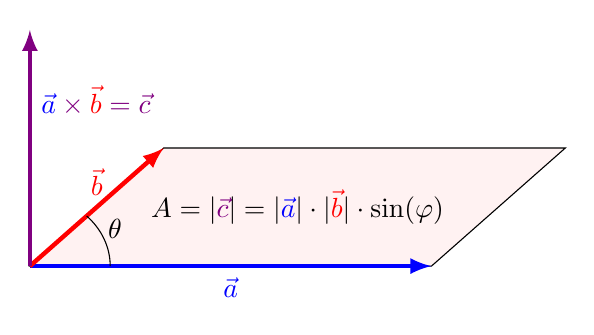
\begin{tikzpicture}[yscale=1.5, xscale=1.7, every node/.style={scale=1}]
    % Rechteck
    \draw[-,fill=white!95!red](0,0)--(3,0)--(4,1)--(1,1)--cycle;
    % Formel in der Fläche
    \node at (2,0.5) {$A = |\textcolor{violet}{\vec{c}} | = |\textcolor{blue}{\vec{a}}| \cdot |\textcolor{red}{\vec{b}}| \cdot \sin(\varphi)$};
    % a
    \draw[ultra thick,-latex,blue](0,0)--(3,0)node[midway,below]{$\vec{a}$};
    % b
    \draw[ultra thick,-latex,red](0,0)--(1,1)node[midway,above]{$\vec{b}$};
    % a x b
    \draw[ultra thick,-latex,blue!50!red](0,0)--(0,2)node[pos=0.7,right]{$\textcolor{blue}{\vec{a}} \times \textcolor{red}{\vec{b}} = \vec{c}$};
    \draw (0.6,0) arc [start angle=0,end angle=45,radius=0.6]
    node[pos=0.7,right]{$\theta$};
    \end{tikzpicture}
\end{minipage}
    \input{../../Snippeds/Vektoranalysis/Nabla.tex}
    \subsubsection{Tangentialebene}
\begin{flalign}
    &z = f(x_0; y_0) + \nabla f_x(x_0; y_0) \cdot (x - x_0) + \nabla f_y(x_0; y_0) \cdot (y - y_0)&\\
    &\vec{n} = \left(\begin{matrix}
        f_x(x_0; y_0)\\
        f_y(x_0; y_0)\\
        -z\\
    \end{matrix}\right)&\label{eq:Normalenvektor}
\end{flalign}
\vspace{4mm}
\ref{eq:Normalenvektor} Normalenvektor, welcher senkrecht auf der Tangentialebene steht\\

\begin{minipage}{0.4\linewidth}
    \textbf{Priorisierung um den Gradienten in die Tangentialebenenform zu bekommen}
    \begin{enumerate}
        \item Faktorisieren
        \item Additionsverfahren
        \item Umstellen und Einsetzen
    \end{enumerate}
\end{minipage}
\hfill
\begin{minipage}{0.4\linewidth}
    \textbf{Beispiel}\\
    \begin{flalign}
        &f(x,y) = x^3 + x^2 \cdot \ln{y^2 + 1} - 3x&\notag\\
        &\nabla f(x,y) = \begin{matrix}
            3x^2 - 2x \cdot \ln{y^2 + 1} - 3\\
            - \frac{2x^2y}{y^2 + 1}
        \end{matrix}&\notag\\
        &f(3;1) = 27 - 9\cdot \ln{2} -9 = 18 - 9\cdot \ln{2}&\notag\\
        &\nabla f_x (3; 1) = 27 - 6\ln{2} - 3 = 24 - 6\ln{2}&\notag\\
        &\nabla f_y(3;1) = -9&\notag\\
        &-45 + 9\ln{2} - 6x\ln{2} + 24x - 9y&\notag
    \end{flalign}
\end{minipage}
    \subsubsection{Totales Differential}
\textbf{Formel für das Totale Differential}\\
\begin{flalign}
    &df = f_x \cdot dx + f_y + \ldots + f_n&\\
    &df = \sum_{i=1}^{n}{f_{x_i} \cdot d_{x_i}}&
\end{flalign}

\textbf{Anleitung für das Totale Differential}\\
\begin{enumerate}
    \item Gradient der Funktion berechnen
    \item Komponenten des Gradienten addieren
    \item Falls benötigt Punkt für Komponenten x,y,.. etc. einsetzen
\end{enumerate}
    \subsubsection{Hessematrix}
\begin{minipage}{0.4\linewidth}
    \begin{flalign}
        &H = \nabla^2f = \left[\begin{matrix}
            f_{,1,1} & f_{,1,2} & \cdots & f_{,1,n}\\
            f_{,2,1} & f_{,2,2} & \cdots & f_{,2,n}\\
            \vdots & \vdots & \ddots & \vdots\\
            f_{,n,1} & f_{,n,2} & \cdots & f_{,n,n}\\
        \end{matrix}\right]&
    \end{flalign}
\end{minipage}
\hfill
\begin{minipage}{0.4\linewidth}
    \textbf{Schwarz-Clairaut-Young-Satz}\\
    \begin{flalign}
        &H = H^T&
    \end{flalign}
\end{minipage}
    \subsubsection{Extremwertstellen/Kritische Stellen}
\textcolor{red}{Lagrange Verfahren einfügen}
\begin{flalign}
    &\text{Kritische Stellen } = \nabla f \stackrel{!}{=} 0&\\
    &L(\vec{x}, \lambda) = f(\vec{x}) + \lambda \cdot g(\vec{x})&\\
    &\nabla L \stackrel{!}{=} 0&\\
\end{flalign}
    \subsection{Matrizen}
    \subsubsection{Standardmatrizen}
\vspace{3mm}
\begin{minipage}{0.4\linewidth}
    \begin{flalign}
        &\mathbb{I} = \left(\begin{matrix}
            1 & 0\\
            0 & 1\\
        \end{matrix}\right)&\\
        &\mathbb{P} = \left(\begin{matrix}
            -1 & 0\\
            0 & -1\\
        \end{matrix}\right)&
    \end{flalign}
\end{minipage}
\hfill
\begin{minipage}{0.5\linewidth}
    \begin{flalign}
        &\mathbb{R_{\alpha}} = \left(\begin{matrix}
            \cos{\varphi} & -\sin{\varphi}\\
            \sin{\varphi} & \cos{\varphi}
        \end{matrix}\right)&\\
        &\mathbb{R_{-\alpha}} = \left(\begin{matrix}
            \cos{\varphi} & \sin{\varphi}\\
            -\sin{\varphi} & \cos{\varphi}
        \end{matrix}\right)&
    \end{flalign}
\end{minipage}
    \subsubsection{Determinante}
\textbf{Regeln}
\begin{itemize}
    \item $\det(A^{T}) = \det(A)$
    \item $\det(a \cdot A^{T}) = a^n \cdot \det(A)$
    \item $\det(A \cdot B) = \det(A) \cdot \det(B)$
    \item $\det(A^{-1}) = \frac{1}{\det(A)}$ falls A regulär
    \item Zeilen-/Spaltentausch\\ $\det(A) \mapsto -\det(A)$
    \item Multiplikation einer Zeile/Spalte mit a\\ $\det(A) \mapsto a \cdot \det(A)$
    \item Invarianz: Subtrahiert man von einer Zeile ein vielfaches einer anderen Zeile, so ändert sich die Determinante nicht
\end{itemize}

\textbf{2x2 Matrizen}\\
\begin{minipage}{0.29\linewidth}
    \vspace{3mm}
    \begin{flalign}
        & \det(
            \begin{matrix}
                $\tikzmarknode{a}{a}$ & $\tikzmarknode{b}{b}$\\
                $\tikzmarknode{c}{c}$ & $\tikzmarknode{d}{d}$\\
            \end{matrix}
        ) = &\notag
    \end{flalign}
    \begin{tikzpicture}[overlay, remember picture]
        \draw[-, red, thick] (a) to (d);
        \draw[-, blue, thick] (c) to (b);
    \end{tikzpicture}
\end{minipage}
\hfill
\begin{minipage}{0.39\linewidth}
    \begin{flalign}
        &\textcolor{red}{(a \cdot d)} - \textcolor{blue}{(c \cdot b)}& \label{eq:2x2_Determinante}
    \end{flalign}
\end{minipage}\\
\textbf{3x3 Matrizen}\\
\begin{minipage}{0.39\linewidth}
    \vspace{3mm}
    \begin{flalign}
        & \det(
            \begin{matrix}
                $\tikzmarknode{a}{a}$ & $\tikzmarknode{b}{b}$ & $\tikzmarknode{c}{c}$\\
                $\tikzmarknode{d}{d}$ & $\tikzmarknode{e}{e}$ & $\tikzmarknode{f}{f}$\\
                $\tikzmarknode{g}{g}$ & $\tikzmarknode{h}{h}$ & $\tikzmarknode{i}{i}$\\
            \end{matrix}
        ) = &\notag
    \end{flalign}
    \begin{tikzpicture}[overlay, remember picture]
        \draw[-, red, thick] (a) to (e) to (i);
        \draw[-, red, thick] (b) to (f) to (g);
        \draw[-, red, thick] (c) to (d) to (h);
        \draw[-, blue, thick] (g) to (e) to (c);
        \draw[-, blue, thick] (h) to (f) to (a);
        \draw[-, blue, thick] (i) to (d) to (b);
    \end{tikzpicture}
\end{minipage}
\hfill
\begin{minipage}{0.59\linewidth}
    \begin{flalign}
        &\textcolor{red}{(a \cdot e \cdot i) + (b \cdot f \cdot g) + (c \cdot d \cdot h)}&\notag\\
        &\textcolor{blue}{- (g \cdot e \cdot c) - (h \cdot f \cdot a) - (i \cdot d \cdot b)}& \label{eq:3x3_Determinante}
    \end{flalign}
\end{minipage}

% Define signed matrix colors
\definecolor{pos-sign}{RGB}{255,0,0}  % Red for '+'
\definecolor{neg-sign}{RGB}{0,0,255}  % Blue for '-'

% Custom command for colored sign entries
\newcommand{\sign}[1]{\if#1+{\color{pos-sign}+}\else{\color{neg-sign}-}\fi}

\textbf{4x4 Matrizen / nxn Matrix}\\
\begin{minipage}{0.3\linewidth}
    \vspace{3mm}
    \begin{flalign}
    &\mathrel{\vcenter{\hbox{
        \begin{tikzpicture}[baseline=(A.base), remember picture]
        % Original coefficient matrix
        \matrix [matrix of nodes, nodes={inner sep=2mm}, anchor=base, left delimiter=(, right delimiter=),
                ampersand replacement=\&] (A) {
            \tikzmarknode{a}{a} \& \tikzmarknode{b}{b} \& \tikzmarknode{c}{c} \& \tikzmarknode{d}{d}\\
            \tikzmarknode{e}{e} \& \tikzmarknode{f}{f} \& \tikzmarknode{g}{g} \& \tikzmarknode{h}{h}\\
            \tikzmarknode{i}{i} \& \tikzmarknode{j}{j} \& \tikzmarknode{k}{k} \& \tikzmarknode{l}{l}\\
            \tikzmarknode{m}{m} \& \tikzmarknode{n}{n} \& \tikzmarknode{o}{o} \& \tikzmarknode{p}{p}\\
        };
        % Overlay sign matrix (transparent)
        \matrix [matrix of nodes, opacity=0.7,
                nodes={inner sep=2mm}, overlay, ampersand replacement=\&,
                shift={(0.2,0.15)}] at (A) {
            \sign{+} \& \sign{-} \& \sign{+} \& \sign{-}\\ 
            \sign{-} \& \sign{+} \& \sign{-} \& \sign{+}\\ 
            \sign{+} \& \sign{-} \& \sign{+} \& \sign{-}\\ 
            \sign{-} \& \sign{+} \& \sign{-} \& \sign{+}\\ 
        };
    \end{tikzpicture}}}} = A^{4x4}&\notag
    \end{flalign}
\end{minipage}
\hfill\hspace{-7mm}
\begin{minipage}{0.6\linewidth}
    \begin{enumerate}
        \item Spalte/Reihe mit den meisten Nullen auswählen
        \item Die Vorfaktoren der Spalten/Reihenwerte mit der Vorzeichenmatrix (\textcolor{red}{+}, \textcolor{blue}{-}) bestimmen
    \end{enumerate}
\end{minipage}

\begin{equation}
    \det(A^{4\times4}) = \overbrace{D_a + D_e + D_i + D_m}^{\boxed{4}} =
        \begin{cases}
            \begin{aligned}
            D_a &= {\color{red}\boxed{+}} a \cdot \det\begin{pmatrix}
                        f & g & h\\ 
                        j & k & l\\
                        n & o & p
                    \end{pmatrix} \\ 
            D_e &= {\color{blue}\boxed{-}} e \cdot \det\begin{pmatrix}
                        b & c & d\\
                        j & k & l\\
                        n & o & p
                    \end{pmatrix} \\
            \boxed{3}\\
            D_i &= {\color{red}\boxed{+}} i \cdot \det\begin{pmatrix}
                        b & c & d\\
                        f & g & h\\ 
                        n & o & p
                    \end{pmatrix} \\
            D_m &= {\color{blue}\boxed{-}} m \cdot \det\begin{pmatrix}
                        b & c & d\\
                        f & g & h\\
                        j & k & l
                    \end{pmatrix}
            \end{aligned}
        \end{cases}
    \label{eq:nxn_Determinante}
\end{equation}
\begin{enumerate}[start=3]
    \item 3x3 Matrizen aufstellen durch abdecken der Zeilen und Spalten des jeweiligen Vorfaktors
    \item Ergebnisse addieren ergibt die Determinante der 4x4 Matrix
\end{enumerate}
    \subsubsection{Inverse berechnen mittels Adjunkter Matrix}
\begin{enumerate}
    \item Determinante berechnen
\end{enumerate}
    \newcommand{\Rang}[1]{Rang{#1}}

\subsubsection{Eigenwerte}
\textbf{Formeln}\\
\begin{flalign}
    &\textbf{Charakteristisches Polynom}&\notag\\
    &p_A(\lambda) = \det(\lambda \cdot \mathds{1} - A)&\label{eq:Char_Polynom}\\
    &p_A(\lambda) = a_n \cdot \lambda^n + a_{n - 1} \cdot \lambda^{n - 1} + \cdots + a_1 \cdot \lambda + a_0&\label{eq:Char_Polynom_ausmultipliziert}\\
    &\textbf{Eigenwertproblem}&\notag\\
    &A\vec{x} = \lambda \cdot \vec{x}, \qquad \vec{x} \ne \vec{0}&\label{eq:Eigenwertproblem}\\
    &\textbf{Wichtiger Satz}&\notag\\
    &\Rang(A) = n \Leftrightarrow \det(A) \ne 0 \Leftrightarrow A^{-1} \nexists &\notag\\
    &\Leftrightarrow A \vec{x} = \vec{0} \leftrightarrow \vec{x} = \vec{0} \Leftrightarrow \lambda = 0 \text{ }\cancel{\in} \operatorname{EW}(A)&
\end{flalign}\\
\textbf{Wichtiges}
\begin{multicols}{2}
    \begin{itemize}
        \item $\lambda$ = Eigenwert
        \item $\vec{x}$ = Eigenvektor
        \item $a_n = 1$
        \item $a_{n-1} = -\tr(A)$
        \item $a_0 = (-1)^n \cdot \det(A)$
    \end{itemize}
\end{multicols}
\textbf{Anleitung}\\
\begin{enumerate}
    \item Gleichung des Charakteristischen Polynoms aufstellen
    \item Determinante berechnen mit einer der folgenden Optionen:\\
        \bullet \ref{eq:3x3_Determinante} 3$\times$3 Determinante - Regel von Sarü\\
        \bullet \ref{eq:nxn_Determinante} N$\times$N Determinante
    \item \ref{eq:Char_Polynom_ausmultipliziert} $\Leftrightarrow$ Charakteristisches Polynom\\
        \bullet Hinterer Teil zusammenfassen\\
        \bullet Grad n \qquad  \bullet Max. n Lösungen\\
        \bullet $n = 2: p_A(\lambda) = \lambda^2 -\tr(A) \cdot \lambda + \det(A)$\\
        \bullet $n = 2$ falls $D > 0$: Mitternachtsformel \ref{eq:Mitternachtsformel}\\
        \bullet $n > 2$ Hornerschema \ref{eq:Hornerschema}
    \item Prüfung der Ergebnisse der Eigenwerte\\
    \bullet $\tr(A) = \sum_{k = n}^{n}{\lambda_k}$ \qquad   \bullet $\det(A) = \prod_{k = n}^{n}{\lambda_k}$\\
    \bullet EW von $A^{-1} = \frac{1}{\lambda}$
    \item Ausrechnen der Eigenvektoren ist bei den Eigenvektoren beschrieben
\end{enumerate}

\begin{flalign*}
    &\boxed{1}: \ref{eq:Eigenwertproblem} \Rightarrow A \vec{x} - \lambda \vec{x} = \vec{0}&\\
    &\ref{eq:Char_Polynom}: (\underbrace{A - \mathds{1} \lambda}_{A}) \vec{x} = \vec{0}&\\
    &\boxed{2}: \det(\overbrace{\begin{pmatrix}
        A_{11} - \lambda_{11} & A_{12} & A_{13}\\
        A_{21} & A_{22} - \lambda_{22} & A_{23}\\
        A_{31} & A_{32} & A_{33} - \lambda_{33}\\
    \end{pmatrix}}^{A}) \vec{x} \stackrel{!}{=} \vec{0}&\\
    &\boxed{3}: \ref{eq:Char_Polynom_ausmultipliziert}: p_A(\lambda) = a_n \cdot \lambda^n + a_{n - 1} \cdot \lambda^{n - 1} + \cdots + a_1 \cdot \lambda + \overbrace{a_0}^{\text{Hinterer Teil}}&\\
\end{flalign*}
\subsubsection{Eigenvektoren}
\textbf{Notwendig für die Berechnung der Eigenvektoren}
\begin{itemize}
    \item Eigenwerte
\end{itemize}
\textbf{Anleitung}\\
\begin{enumerate}
    \item Für jeden Eigenwert eine Tabelle aufstellen mit $A - \lambda_n$ damit es zum Rangverlust kommt
    \item Mittels Gauss links unten Nullen Produzieren
    \item Mittels Treppentrick freie Parameter bestimmen
    \item Einsetzen
    \item Faktor aus/rein multiplizieren, damit es ein ganzzahligen EW gibt
\end{enumerate}

\begin{flalign*}
    &\boxed{1}: \textbf{Eigenvektor zu $\lambda_i$}&\\
    &\boxed{2}: \begin{tabular}{*{3}{>{$}r<{$}|} >{$}r<{$}}
        x & y & z & 0\\ 
            \hline
        A_{11} - \lambda_i & A_{12} & A_{13} & 0\\
        A_{21} & A_{22} - \lambda_i & A_{23} & 0\\
        A_{31} & A_{32} & A_{33} - \lambda_i & 0\\
    \end{tabular}&\\
    &\qquad \qquad \qquad \vdots&\\
    &\boxed{3}: \begin{tabular}{*{3}{>{$}r<{$}|} >{$}r<{$}}
        x & y & z & 0\\ 
            \hline
        \boxed{A_{11} - \lambda_i} & A_{12} & A_{13} & 0\\
        \cline{1-1}
        0 & \boxed{A_{22} - \lambda_i} & A_{23} & 0\\
        \cline{2-2}
        0 & 0 & \boxed{A_{33} - \lambda_i} & 0\\
        \cline{3-3}
    \end{tabular}&\\
    &\boxed{4}: \begin{pmatrix}
        t \cdot x\\
        t \cdot y\\
        t
    \end{pmatrix} \Rightarrow \boxed{5}: t \cdot \begin{pmatrix}
        x\\
        y\\
        1
    \end{pmatrix}, t \in \mathds{R}\backslash \{0\}&
\end{flalign*}
    Die Spur:
Alle Einträge der Matrix auf der Diagonalen summiert.

Aussagefähigkeit:
- $trace(A) = \sum_{0}^{n}{\lambda_{n}}$
- 
}
\end{document}